\ifgerman{\chapter{Implementation}}{\chapter{Implementation}}

This chapter describe in detail about how data was collected, what preprocessing techniques were applied to the data in order to make it fit for machine learning algorithm to learn from, how data was resampled in order to balance it to some extent, how it was clustered and what are the details of the architecture of the models and what are the evaluation strategies applied.

\section{Data Collection}
To begin with the implementation, the first step was to obtain the data. Obtaining the data was particularly  challenging as these summaries were frequently changing, so scrapping the data at different times results in different assignment of a single document in different categories. Also another challenge was that when documents for English and German were scraped separately, it happened quite often that some documents from one language were missing. Due to these challenges, a carefully crafted scraper which scrapes the data only if documents from both the languages are available, this in turn added a time overhead. Even after those considerations, there were some documents missing from one of the language.

For scrapping the data Python library \textit{Beautiful Soup} and \textit{urllib} was used. 

\section{Data Cleaning}\label{preprocessing}

The preprocessing involved removing of \textit{punctuation's}, \textit{numbers}, \textit{currency symbols} as they do not contribute anything in the classification process. The next step is to normalize the text, this step is necessary because of the \textit{inflection} added due to the modification of words.

%\todo{A figure explaining how played, plays and playing is all from the root word \textit{play} }
Stemming and Lemmatization are two techniques used to normalize the text. Both techniques reduces words to its root form. Stemming reduces the word into base but this base may or may not be the morphological root of the word. It should suffice that the related words are mapped to the same base, even if the base is not a valid root. For example, words \textit{argued}, \textit{arguing}, \textit{argue} and \textit{argues} will all be stemmed to \textit{argu}, even though the base \textit{argu} is not a valid term in itself. The process of stemming is more heuristic. It removes affixes such as \textit{-ed,-ize, -s,-de} without taking into account that the base might not be a word in the same language. On the contrary lemmatization reduces the words by ensuring that the base belong to the language. The base word in lemmatization is called a \textit{lemma}. Lemmatization is necessary in the cases where it is necessary to get valid words.This will be clear in the coming section of word embeddings. This is the reason, that instead of stemming, lemmatization is used as word normalization technique.  \todo{example of lemmatization and stemming comparision}

As the last step, \textit{stop words} from both the languages were removed because, first they don't contribute anything, second they increase the training time of the algorithm. For German language, \textit{umlauts - ä, ö and ü} are converted into its base form that is \textit{ä to ae, ö to oe and ü to ue.}

Following are the steps in which the preprocessing was done.

\begin{enumerate}
    \item As a first step, \textit{stop words} are removed.
    \item Next step is to lemmatize the words.
    \item Removal of other unnecessary symbols are removed. For example, § is symbol of paragraph and is extensively used in legal text. • is also another example.
    \item Remove numbers
    \item Punctuation removal
\end{enumerate}

The order of the steps is also important as it will help in reducing the overload on some of the processes. For example, when the stop words are removed in the first step, then the lemmatizer would not have to go through those words and that will decrease the time taken to process the text. There were other Unicode characters which were also removed. 

\subsection{Data Preprocessing for pretrained word embeddings}
Pretrained language models are trained on large corpora and hence they can be used for variety of task in natural language processing. These models are trained on corpora that have no specific domain. Legal text is different from the corpora these models are trained on such that the words we find in legal text are rarely used outside the legal domain. 

For the scope of this thesis, to answer the question \textit{"Can general purpose resource be used for legal domain specific task?"} I am going to use Facebook's MUSE multilingual word embeddings \cite{conneau2017word}. These word embeddings are created by learning a mapping between the two sets of monolingual word embeddings.\todo{have to write what methods were used to create these} The monolingual word embedding used in were created using fastText \cite{bojanowski2017enriching}. These pretrained vectors were trained on Common Crawl and Wikipedia Coprus. There was no preprocessing involved except for lower casing the words. Hence, to use these word embeddings, I need to use the corpus with only lower case words and avoid all the preprocessing mentioned in the section in order to have the classifier learn better. If the preprocessed data is used with the embedding that were created using non processed data then even if the 


\section{Data Resampling} \label{dataResampling}
The EUR-Lex summaries, are the summarised versions of legislations. These summaries are written in an abstract manner to apply for multiple situations, so that one regulation may belong to several categories. Multi-label classifier with very few examples might not be applicable as the classifier will favour majority class because of the imbalance. 

From \ref{graph:distribution of data english docs} it is clear that the data suffers from class imbalance. To mitigate the problem of class imbalance we upsample minority class or downsample majority class. In our case, upsampling minority class is difficult as it is very hard to produce alike documents because of nature of text and downsampling minority class would lessen the already less data. We had to find a way to not only downsample the majority in such a fashion that would result into balancing the data as well as not lessen the data to an extent that is not useful anymore.
\todo{give an example to make it clear}
As the data is multilabeled it can be exploit because of the fact that a sample might belong to more than one class. The documents are transformed in such a way that if a document belongs to two or more class, then it will be kept in the class with minimum number of samples. That is the class label for that document will be the one with the fewest examples. This method will downsample the majority class as only the duplicated documents are removed from it but also make this classification problem a multi-class from a multi-label one. In the testing phase, the predictions are allowed from the set of all the true labels. This method however introduces a bais towards the minority classes but it acknowledges the presence of other possible category assignment in the end result.

\begin{figure}[!ht]
\begin{center}
\makebox[2pt]{
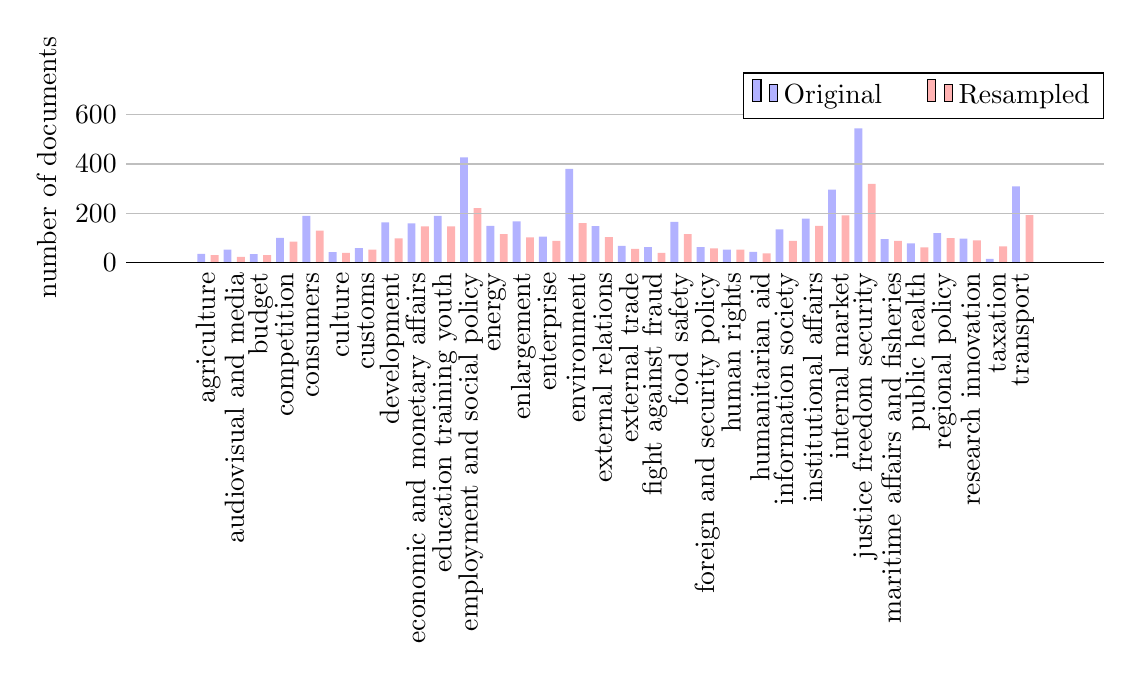
\begin{tikzpicture}
  \centering
  \begin{axis}[
        ybar, axis on top,
        title={},
        height=4cm, width=14cm,
        bar width=0.1cm,
        ymajorgrids, tick align=inside,
        enlarge y limits={value=.1,upper},
        ymin=0, ymax=700,
        axis x line*=bottom,
        axis y line*=left,
        y axis line style={opacity=0},
        tickwidth=0pt,
        ytick style={draw=none},
        enlarge x limits=true,
        legend style={
            at={(1,1)},
            anchor=north east,
            legend columns=-1,
            /tikz/every even column/.append style={column sep=0.5cm}
        },
        ylabel={number of documents},
        symbolic x coords={
        agriculture,
        audiovisual  and  media,
        budget,
        competition,
        consumers,
        culture,
        customs,
        development,
        economic  and  monetary  affairs,
        education  training  youth,
        employment  and  social  policy,
        energy,
        enlargement,
        enterprise,
        environment,
        external  relations,
        external  trade,
        fight  against  fraud,
        food  safety,
        foreign  and  security  policy,
        human  rights,
        humanitarian  aid,
        information  society,
        institutional  affairs,
        internal  market,
        justice  freedom  security,
        maritime  affairs  and  fisheries,
        public  health,
        regional  policy,
        research  innovation,
        taxation,
        transport
        },
       xtick=data,
       x tick label style={rotate=90,anchor=east},
       %nodes near coords={\pgfmathprintnumber[precision=0]{\pgfplotspointmeta}}
    ]
    \addplot [draw=none, fill=blue!30] coordinates {
        (agriculture, 37)
	    (audiovisual and media,54) 
		(budget,36) 
		(competition,101) 
		(consumers,190) 
		(culture,44) 
		(customs,60) 
		(development,164) 
		(economic and monetary affairs,160) 
		(education training youth,190) 
		(employment and social policy,427)
		(energy,150)
		(enlargement,168)
		(enterprise,106)
		(environment,380)
		(external relations,149)
		(external trade,69)
		(fight against fraud,64)
		(food safety,166)
		(foreign and security policy,64)
		(human rights,54)
		(humanitarian aid,45)
		(information society,136)
		(institutional affairs,179)
		(internal market,296)
		(justice freedom security,544)
		(maritime affairs and fisheries,96)
		(public health, 79)
		(regional policy,120)
		(research innovation,98)
		(taxation,16)
		(transport,309)  };
   \addplot [draw=none,fill=red!30] coordinates {
      (agriculture, 32)
(audiovisual and media, 24)
(budget, 32)
(competition, 86)
(consumers, 131)
(culture, 41)
(customs, 54)
(development, 99)
(economic and monetary affairs, 148)
(education training youth, 148)
(employment and social policy, 222)
(energy, 116)
(enlargement, 103)
(enterprise, 89)
(environment, 161)
(external relations, 104)
(external trade, 57)
(fight against fraud, 41)
(food safety, 116)
(foreign and security policy, 59)
(human rights, 54)
(humanitarian aid, 39)
(information society, 89)
(institutional affairs, 150)
(internal market, 192)
(justice freedom security, 320)
(maritime affairs and fisheries, 89)
(public health, 63)
(regional policy, 100)
(research innovation, 91)
(taxation, 67)
(transport, 193) };
\legend{Original, Resampled}
\end{axis}
\end{tikzpicture}
}
\end{center}
\captionsetup{justification=centering,margin=2cm}
\caption{Class distribution of the EUR-Lex summaries corpus, comparing the original
to the resampled distribution.}
\label{graph:originalVSresampled}
\end{figure}


\section{Clustering} \label{clustering}
Document cluster in information retrieval helps in organization, extraction of topic and text, filtering. The idea here was that given the number of classes and the number of documents per classes as it is a unbalanced dataset,it will be difficult for a classifier to learn on this data. 

Clustering of documents was only possible provided that all the documents $d$ of a category $C$ belong only to that category. Also, it is important to find out what is the number $n$ that the documents must be clustered into. The number of clusters $n$ is determined bu silhouette score \cite{rousseeuw1987silhouettes} and elbow analysis \cite{thorndike1953belongs}. 

K-Means cluster is used here to cluster the documents. Splitting the documents this way, the number of classes to be predicted by each classifier is reduced thus, resulting in specialization advantage for each classifier. However, the final classification depends on the classification from previous classifiers, so any error introduced will be propagated downwards. This method of division is can be advantageous as we have $32$ classes and it can be a challenge for a single classifier to learn on them given the amount of data.

\clearpage


\section{Training the Word Vectors}

Conventionally, text representation in natural language processing involves techniques like \textit{Continuous bag-of-words} and \textit{if-idf}. These techniques are simple representation of various features. However, in bag-of-words approach, grammar and word order are not considered. And in tf-idf only importance of words is considered, section \ref{sec:svm}. Hence, techniques does not capture the semantics of the text \cite{maas2011learning}.

\todo{already in backgroud, write about just the training part. How you did it}
Due to the above limitations words vectors are used. Word embeddings are vector representation of meaning of words in the corpus. This means that words are placed in high-dimensional vector space where words with similar meaning are placed close to each other. Neural network based word vector models are usually trained using stocastic gradient descent where gradient is obtained by backpropogation \cite{le2014distributed}. One popular algorithm is \textbf{Word2Vec} \cite{mikolov2013efficient},in this implementation word embedding are trained using two models, Continuous bag-of-word model and Continuous Skip-gram model. In continuous bag-of-words, the projection of words into vector space is not influenced by the order of words and words from future are also used in this model. Unlike, standard bag-of-words it uses continuous distributed representation of context. The architecture is similar to Feedforward Neural Net Language model \cite{bengio2003neural}. In Continuous Skip-gram model, instead of predicting next word based on context, it tries to maximize the classification of next word based on other word in the sentence.

After the network converges, words with similar meaning are placed together. For example words like "powerful" and "strong" are placed closed in the vector space. \todo{Need to work on this, doesn't look good}

The model used in creation of the word vectors is a neural network, and neural networks are data hungry as it requires a lot of data to train them properly. As a result, another domain specific dataset is used in this experiment because dataset used for classification is small. Hence, the whole EUR-Lex dataset was used as it contains 19,348 documents mostly consisting regulations, decisions and directives of European Union \cite{jf:SemanticLaw}.

\subsection{Cross Lingual Word Embedding}
Word vectors for different languages are in different vector spaces, hence it can not be combined together, but the classification task involves classifying text from two languages, \textbf{English} and \textbf{German}. Hence, for classifying both languages within a single model is necessary. This not only mitigates the error caused by a language detector in multilingual systems, where a language detector first detects the language and then the respective classifier is invoked. In that affair, error propagates downwards and amplifies. And using multiple languages also increase the amount of data for training if multilingual parallel corpora is available where corpus of single language is low. 

To achieve this \cite{duong2016learning}, proposed using bilingual dictionaries and monolingual data. The model uses an extension of contextual bag-of-word(CBOW) model \cite{mikolov2013efficient}. This method has benefits as often there no parallel data when working on a domain specific problems, also it is comparatively easy to obtain or create bilingual domain specific dictionaries. \todo{Write about the method}

I will be using the technique suggested by \cite{duong2016learning}. For creating bilingual dictionary, \textit{EuroVoc} thesaurus \cite{steinberger2002cross} provided by Publication office of European Union will be used. It is available in 24 official languages recognised by European Union. This thesaurus is domain specific hence it does not involve common words that might occur in the documents. Due to this reason, this thesaurus is combined with bilingual dictionaries that are available from \textit{Facebook MUSE} \cite{conneau2017word}. This bilingual dictonaries were created using Facebook's internal translation tools. The authors claims that these dictionaries handle the polysemy of the words better. This combined bilingual dictionary with the original EUR-Lex dataset was used to create the legal domain specific bilingual word embeddings. 

For creating General purpose word embedding using the above mention method is time and resource consuming, as a lot of monolingual data needs to be obtained and also large bilingual dictonaries need to be obtained as well. This would also mean that there would be bais in creation of these embeddings as we would have prior knowledge about what works well with algorithms and the data we are using, also this would beat the purpose of comparing General Purpose resources to one created using domain specific resources. Hence, we are using Facebook's MUSE word embeddings \cite{conneau2017word}, the author claims that the embeddings are state-of-art multilingual word embeddings, these word embedding are facebooks fasttext \cite{bojanowski2017enriching} which are aligned in common vector space. They use two sets word embeddings that are trained on monolingual data, and learns the mapping between these two embedding in a common vector space. It exploits the similarities of monolingual embedding space \cite{mikolov2013exploiting} to learn mapping between the two embeddings.
The method used by \cite{conneau2017word} is domain adversarial learning. \todo{this needs to go} In this method a model is trained to discriminate between randomly sampled elements from the two embeddings. For example, let $X$ $=$ ${x_{1}, x_{2}...x_{n}}$ be the first of the two monolingual word embedding, and $Y$ $=$ ${y_{1}, y_{2}...,y_{n}}$ be the second monolingual word embedding. $W$ is trained to block the discriminator making right predictions. 


\section{Architecture and Training}

The case of class imbalance is clear from \ref{graph:distribution of data english docs}. Applying the resampling technique proposed in \ref{dataResampling}, we have mitigated the problem of data imbalance to some extent. The \ref{fig:approach} shows the divide-and-conquer philosophy. This approach assumes that the classifier will benefit from the specialization effect from a small number of classes. \\

\begin{figure}[!ht]
    \centering
    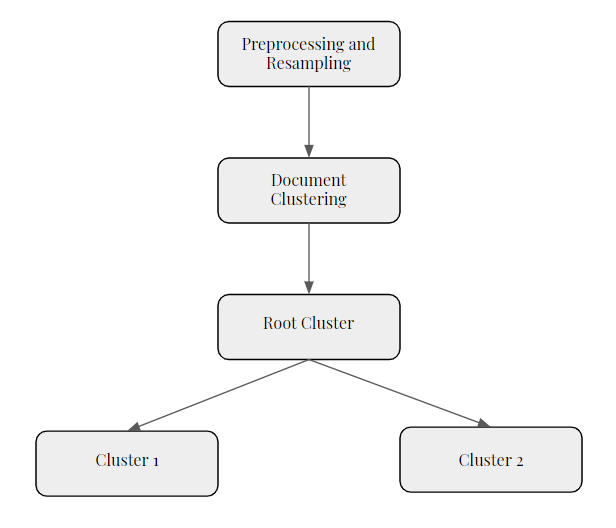
\includegraphics[height=5cm,width=9cm,keepaspectratio]{pics/Approach.PNG}
    \captionsetup{justification=centering,margin=2cm}
    \caption{The workflow of the preparation, resampling and training of the proposed technique.}
    \label{fig:approach}
\end{figure}
\clearpage

First the preprocessing of the documents is done, after that in the resampling phase, class imbalance is tackled to some extent. Then, similar categories are grouped together based on the clustering technique presented in \ref{clustering}. In the data set preparation stage, the English and German documents with labels were pickled together so that during the Train-Test split, no parallel document from either language ends up in both, that is if \textbf{Doc A} from English language and parallel document \textbf{Doc} $\mathbf{\Tilde{A}}$ from German language don't end up in Train set and Test set respectively or vice versa. After ensuring the conformity, the dataset was divided into Train set and Test set with ratio of 70\% and 30\% respectively. This division was done on document level before creating sentences to ensure that sentences from a single document end up in only one of the two sets, This is very important, not conforming to this might create problem of data leakage. Also the train-test split was performed in stratified fashion to ensure that the ratio of number of samples in classes in Train set is same as the ratio of samples of classes in Test set.
















